\subsection{Inspiration}
The inspiration for this project came directly from the paper, "Picking Winners" written by David Hunter, et al. The paper targets "top heavy" daily fantasy hockey competitions and uses the integer programming (IP) optimization technique to try to "beat" them. The optimization technique involved the researchers coming up with ideas about what \textit{could} be beneficial for a line-up, building a model around the idea, and then optimizing and testing it. For example, one of their ideas was related to choosing defencemen on the same team. Upon reading this paper, we felt that the same goal could be achieved while allocating more to the computer. The neural net aimed to solve this. 

\subsection{Neural Networks}
%TODO here we should have a (bit) of background on neural networks. Basically like why we thought they would be a good fit for this. Talk about research etc.
As we began exploring machine learning techniques, we decided, through the help of our research as well as our supervisor, that neural networks would allow for a good first implementation of our system. Neural networks are a set of interconnected nodes \cite{neural_net}. Inputs to the neural network are turned to outputs by passing them through a series of functions \cite{neural_net}. Figure \ref{fig:neural_net} below gives an illustrative view of a neural network. The architecture of neural networks is inspired by the structure of a human brain, where the nodes represent neurons, and the links that connect the nodes represent synapses \cite{neural_net}.

\begin{figure}[ht]
    \centering
    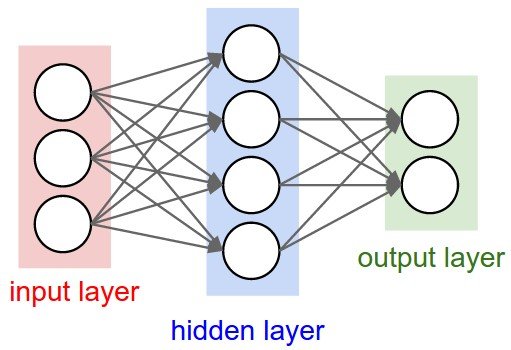
\includegraphics[width=0.50\textwidth]{figures/neural_net}
    \caption{Illustration of neural network \cite{neural_net} }
    \label{fig:neural_net}
\end{figure}

As shown in Figure \ref{fig:neural_net}, a neural network consists of an input layer, an output layer, and one or more hidden layers. Not surprisingly, the input layer takes in the inputs to the system, and the output layer yields the outputs of the system. For example, the input to a particular neural network might be two basketball teams, and the output might be the team we expect to win the match. The question remains, however, how the neural network figures out which output to generate based on a given input. This is done through the help of the hidden layer(s), as well as the links that connect all the nodes \cite{neural_net_fundies}. The combined effort of these two components are what allow learning to take place in a neural network.

In doing our research, we had to ask ourselves whether machine learning, and neural networks in particular, would be appropriate as a means of solving our particular problem. As we found while watching a lecture series on machine learning by Professor Yaser Abu-Mostafa, there are three conditions that should be met in order for machine learning to be considered a viable option \cite{caltech}. First, there needs to be a distinguishable pattern between the inputs and the outputs of the system. For our problem, we hypothesized that this condition would be met since there should be a relationship between the players playing and the outcomes of the games. Secondly, this relationship should not be able to be trivially represented mathematically. This we also thought would be true since there are so many variables at play in any given basketball game. Finally, there needs to be enough data for the neural network to train with. Again, this condition was found to be satisfied. 

Seeing as all three conditions described were satisfied, we deemed neural networks to be an appropriate solution for the matter. In theory, sufficient training of the network should allow learning to take place such that it be able to solve our problem of accurately predicting high-performing fantasy basketball lineups.